\documentclass{article} % For LaTeX2e
\usepackage{nips15submit_e,times}
\usepackage{hyperref}
\usepackage{url}
\usepackage{graphicx}
\usepackage{amsmath,amssymb}
\usepackage{booktabs}
\usepackage{xcolor}
\usepackage[numbers,sort&compress]{natbib}
\usepackage[section]{placeins} % keep each figure/table inside its own section

% TODO markers (remove \todo{...} before submitting; \renewcommand{\todo}[1]{} hides them all)
\newcommand{\todo}[1]{{\color{red}[TODO: #1]}}
\newcommand{\inprogress}{{\color{orange}\textbf{[IN PROGRESS]}}}

\title{Selective Fine-Tuning for Context Distillation}

\author{
Arshia Nayebnazar \\
UC Berkeley \\
arshian@berkeley.edu \\
\And
Yash Saxena \\
UC Berkeley \\
yash\_saxena@berkeley.edu \\
\AND
Michael Liu \\
UC Berkeley \\
liu.michael@berkeley.edu \\
\And
Evan Luo \\
UC Berkeley \\
evan-luo@berkeley.edu \\
}

\newcommand{\fix}{\marginpar{FIX}}
\newcommand{\new}{\marginpar{NEW}}

\nipsfinalcopy % show author names (class report, not anonymous)

\begin{document}

\maketitle

% =====================================================================================================
\begin{abstract}
In-context learning (ICL) enhances the capabilities of Large Language Models (LLMs) by teaching knowledge or reasoning through context tokens in the prompt. Context Distillation (CD) is the concept of ``internalizing'' these capabilities by fine-tuning a \emph{student} model (without context) on the outputs of a \emph{teacher} model (with context) so that the student no longer requires that context in the prompt. However, CD methods typically involve full-parameter fine-tuning, which is costly to run for every new piece of context and is prone to catastrophic forgetting. Meanwhile, many recent works in fine-tuning outside CD have demonstrated that selective fine-tuning can achieve the same gains as full-parameter fine-tuning by updating only a small fraction of the weights. In this work, we explore selective fine-tuning (updating between 0.0001\% and 4.2\% of weights) with supervised fine-tuning (SFT) for CD in each of three different ICL task-types: knowledge retrieval, label mapping, and reasoning. In Qwen3.5-0.8B, ICL performance could be nearly fully restored by adjusting less than 1\% of weights in all task types considered, using 2x less peak memory during training. We also find that selecting the right learning rate can mitigate forgetting in out-of-distribution tasks while maintaining near-teacher performance, and structured weight selection does not improve performance over individual weight selection.
\end{abstract}

% =====================================================================================================
\section{Introduction}
\label{sec:intro}

A Large Language Model (LLM) can learn from a set of information through context tokens to enhance its response. This paradigm is commonly referred to as in-context learning (ICL), which allows an LLM to learn directly from the context without needing to further train the model. However, an LLM relying on ICL needs to reprocess the context again for each query and conversation, which is an inefficient use of prompt space and does not inherently make the model better. Context Distillation (CD) refers to the concept of transferring what is learned in the context into the weights of the model, typically by fine-tuning a student model without the context using the outputs of a teacher model with the context. Many approaches involve full fine-tuning or are expensive. Therefore, we were interested in exploring if we could recover ICL performance by tuning only a small fraction of weights. Given the breadth of applications for ICL, we compare this across many different ``task-types,'' including Knowledge Retrieval, Label Mapping, and Mathematical Reasoning. Fine-tuning typically also leads to catastrophic forgetting, so we measure forgetfulness across sparsity levels for each task as well. Our contributions could be summarized as follows:

%\todo{Contributions, as a list:
%(1) a sparsity sweep over six orders of magnitude on three task types;
%(2) evidence that forgetting tracks update size, and a learning-rate rule that limits it;
%(3) cost measurements against full fine-tuning;
%(4) a comparison of individual weights, rows and blocks at a fixed budget.}

% In this paper, we:

% \begin{list}{}{} 
%     \item Perform a sparsity sweep over six orders of magnitude of percentage of weights trained for three tasks
%     \item Show that the size of the learning rate is proportional to the amount a model forgets
%     \item Show that for a given weight sparsity a specific learning rate can be chosen that maximizes task performance while minimizing forgetting on MMLU and math tasks
%     \item Show the cost savings of each approach compared to full fine-tuning
%     \item Compare models on which selective CD of individual weights, rows, and blocks at a fixed budget have been performed
% \end{list}

%In this paper, we make the following contributions:
\begin{itemize}
    \item \textbf{Sparsity sweep:} Evaluate selective CD across six levels of magnitude of updated weights ($0.0001\%$--$4.2\%$) on three ICL task types.
    \item \textbf{Forgetting and learning rate:} Show that forgetting scales with update size via the learning rate, and give a validation-based rule that recovers full ICL performance while limiting forgetting on MMLU and MATH.
    \item \textbf{Efficiency analysis:} Measure the training memory and inference-time prompt savings of selective CD compared to full fine-tuning.
    \item \textbf{Granularity comparison:} Compare individual weight, row, and transformer-block selection at a fixed $4.2\%$ parameter budget.
\end{itemize}

% =====================================================================================================
\section{Background and related work}
\label{sec:related}
% \todo{2--3 pages in total. Each subsection: what is known, closest papers in detail, how we differ.}

\subsection{In-context learning}
%\todo{ICL \citep{brown2020language}; what demonstrations contribute \citep{min2022rethinking};
%learning arbitrary (semantically unrelated) label mappings from context \citep{wei2023larger} --- our
%Label Mapping task follows this.}

ICL was first popularized as a method that used few-shot prompting in context to improve the performance of a frozen language model \citep{brown2020language}. In ICL, the label space, input distribution, and formatting in few-shot prompting matters more than the correctness of the few-shot examples, as even incorrect few-shot prompts still result in nearly intact output \citep{min2022rethinking}. The extent to which an LLM is adaptable to these kinds of changes depends on the size of the model. Smaller models memorize individual semantic mappings between words and ignore swapped labels; however, larger models are able to understand semantic mappings between words in cases like these and are able to have their outputs reflect information provided by the swapped labels in few-shot prompts \citep{wei2023larger}. Our Label Mapping task measures a model's adaptation ability in this way. While these papers focus on how ICL influences LLM output, we focus more so on how to store context in the weights, rather than ICL.

\subsection{Context distillation}
%\todo{\citet{askell2021general} distill a prompt into weights; %\citet{snell2022learning} distill
%instructions, scratchpads and examples. We ask how many weights this needs.}

The first version of context distillation (CD) used a teacher with an alignment prompt in its context to fine-tune a student model, aligning the behavior of the student through distillation \citep{askell2021general}. This approach of performing CD was later generalized for any context beyond just the alignment prompt in the context \citep{snell2022learning}. However, context distillation itself is computationally inefficient, especially for every new piece of context and fine-tuning all parameters in a model. One of our major focuses is on efficiency, by asking how few weights CD actually needs fine-tuned to restore the performance of a model with ICL.


\subsection{Parameter-efficient and sparse fine-tuning}
%\todo{Adapters \citep{houlsby2019parameter}, LoRA \citep{hu2022lora}, BitFit \citep{zaken2022bitfit};
%sparse updates: diff pruning \citep{guo2021diffpruning}, Fisher-based fixed masks \citep{sung2021fish},
%lottery-ticket sparse fine-tuning \citep{ansell2022composable}, scaling sparse fine-tuning to LLMs
%\citep{ansell2024spiel}; skill localization with few parameters \citep{panigrahi2023skill}.
%Our selection: top gradient magnitude, at weight / row / block granularity.
%Can also mention Doc-to-Lora as a much more inefficent method}

Parameter-efficient fine-tuning (PEFT) adapts pretrained models by updating a small subset of parameters, either through added modules such as Adapters \citep{houlsby2019parameter}, low-rank updates such as LoRA \citep{hu2022lora}, or bias-only tuning (BitFit; \citealp{zaken2022bitfit}). For CD, Doc-to-LoRA \citep{charakorn2026doctolora} uses a meta-trained hypernetwork to generate LoRA adapters from a document, but incurs substantial upfront training and architectural overhead. Alternatively, sparse fine-tuning updates a sparse subset of existing weights with no inference overhead, using $L_0$-regularized diff pruning \citep{guo2021diffpruning}, fixed Fisher-information masks \citep{sung2021fish}, lottery-ticket subnetworks \citep{ansell2022composable}, or memory-efficient sparse delta tracking for LLMs \citep{ansell2024spiel}. Relatedly, \citet{panigrahi2023skill} show that task skills localize to as few as $\sim 0.01\%$ of fine-tuned parameters. We build on this line by selecting weights via top gradient magnitude for CD across individual weight, row, and block granularities.

\subsection{Forgetting during fine-tuning}
%\todo{Catastrophic forgetting \citep{mccloskey1989catastrophic,kirkpatrick2017ewc};
%in LLM fine-tuning \citep{luo2023forgetting}; ``LoRA learns less and forgets less''
%\citep{biderman2024lora} --- closest to our finding that update size, not parameter count, drives forgetting.}

Adapting neural networks to new tasks often degrades prior capabilities, a phenomenon known as catastrophic forgetting \citep{mccloskey1989catastrophic}, which methods like Elastic Weight Consolidation mitigate by penalizing changes to important weights \citep{kirkpatrick2017ewc}. Similar degradation occurs during LLM fine-tuning \citep{luo2023forgetting}. Closest to our work, \citet{biderman2024lora} find that LoRA ``learns less and forgets less'' than full fine-tuning by keeping updates closer to the pretrained weights. In sparse CD, we show that forgetting on MMLU and MATH is driven by update magnitude $\|\Delta\theta\|_2$ rather than parameter count alone, and can be controlled via the learning rate without losing ICL recovery.

%\subsection{FADE FOR NOW: Where knowledge lives in transformers}
%\todo{Knowledge neurons \citep{dai2022knowledge}, ROME \citep{meng2022rome}: facts localize in MLP
%weights --- relevant to why knowledge needs more weights than the method task.}

%\subsection{How this work differs}
%\todo{One paragraph: same model, same data, change one factor at a time (share, then granularity);
%forgetting measured on both knowledge (MMLU) and reasoning (MATH).}
% =====================================================================================================
\section{Methods}
\label{sec:methods}

\subsection{Setup and notation}

We use Qwen3.5-0.8B in non-thinking mode as both teacher and student. Each of the task-types we study provides a context $c$ and a set of queries. The \emph{teacher} is the model given the context:
for each training query $x_i$ it produces an answer $y_i = f_\theta(c, x_i)$ by greedy decoding,
giving a training set $\{(x_i, y_i)\}_{i=1}^{n}$, where $y_{i,t}$ is the $t$-th token of answer $i$
($500$ per context). The \emph{student} is the same model without the context. It is fine-tuned
to reproduce the teacher's answers from the query without context  by minimizing the cross-entropy of the teacher's answer tokens:



\begin{equation}
  \mathcal{L}(\theta) = -\frac{1}{\sum_i |y_i|}\sum_{i}\sum_{t=1}^{|y_i|} \log f_\theta\big(y_{i,t} \mid x_i, y_{i,<t}\big)
  \label{eq:sft}
\end{equation}




The prompt (system message and query) is part of the
input but is not predicted. Minimizing Eq.~\ref{eq:sft} is equivalent to maximizing the likelihood
of the teacher's answers. If training succeeds, the student answers new queries as the teacher
would, without reading the context.

\subsection{Tasks}

Our first task-type is knowledge retrieval, in which models are taught fact-based knowledge through ICL. In this work, we synthetically generate fictional context involving 5 facts about 10 different people (e.g. ``Nelost Shoshonel was born in 1991 in the town of Ostzarbrook.''). We synthetically generate a total of 3 different contexts, each with fictional facts about a different set of 10 unique people.

Our second task-type is label-mapping, where the model is asked to classify an input article. The labels themselves are synthetic, and they can only be learned with in-context examples. In this paper, we provide a news article as input and ask the model to classify it. Like the knowledge retrieval task-type, there are 3 separate contexts: the first takes news articles from AG News and the next two from DBpedia. Each context's class are mapped to a different, random label (e.g. for context 1, ``World'' to ``river'', ``Sports'' to ``stone'', ``Business'' to ``cloud'', ``Sci/Tech'' to ``lamp''). The student has to learn these new classification label mappings and apply them to new input articles.

Our final task type is mathematical reasoning, which involves describing worked examples of how to solve a particular kind of problem through the context. Here, the reasoning task is finding the remainder when N is divided by 9. This is our only context for our mathematical reasoning task-type, largely due to the difficulty of teaching reasoning through ICL. This problem in particular led to noticeable performance improvements between the teacher and untrained model, however (79.2\% versus 45.8\%), and was considered in this study.

Examples are in Appendix~\ref{app:tasks}.

\begin{table}[t]
  \centering\small
  \begin{tabular}{lrrrr}
\toprule
Task & Contexts & Val / test per context & Without context & With context (teacher) \\
\midrule
Knowledge Retrieval & 3 & 100 / 200 & 0.0\% & 99.0\% \\
Label Mapping & 3 & 100 / 200 & 0.0\% & 48.2\% \\
Mathematical Reasoning & 1 & 300 / 500 & 45.8\% & 79.2\% \\
\bottomrule
\end{tabular}

  \caption{Task sizes and test accuracy before fine-tuning, with and without context. Accuracies are averaged across contexts.}
  \label{tab:tasks}
\end{table}

\subsection{Selecting weights}

The eligible weights include all linear-layer weights in the transformer blocks ($N = 497.6$M parameters), whereas embeddings, norms, and the LM head were excluded to prevent shortcuts in which parameters that directly affect individual token logits are selected. Weights are scored by their mean absolute gradient of the SFT distillation loss (Eq.~\ref{eq:sft}) across $B = 8$ training batches.

\begin{equation}
  s_j = \frac{1}{B}\sum_{b=1}^{B} \big| \nabla_{\theta_j} \mathcal{L}_b(\theta) \big|
  \label{eq:score}
\end{equation}

Where $B$ is the number of batches, $\theta_{j}$ is the parameter at index $j$, and $s_{j}$ is the score representing its importance to the loss. At each sparsity level, $\rho$, we select the top $\rho N$ weights with the highest scores. For our granularity analysis, we rank output rows by their mean score of their weights and add rows until $\rho N$ weights are reached. Likewise, we rank transformer blocks by mean score and keep whole blocks, where one block is $4.2\%$. Therefore, granularities are matched in parameter count at $\rho=4.2\%$ and are directly comparable.

\subsection{Training}
We train for three epochs using AdamW \citep{loshchilov2019adamw} with zero weight decay and a
batch size of 16, accumulating gradients over micro-batches of four. We use a cosine learning-rate
schedule with 5\% warmup and clip the gradient norm at 1.0. For individual weights and rows, we
freeze the base model and learn additive updates only at the selected positions. For blocks, we
directly update the eligible linear-layer weights in the selected blocks. The selection stays fixed
throughout training, and all unselected parameters remain unchanged. We use bfloat16 autocast
with float32 weights and trainable updates.

\subsection{Evaluation}
All student evaluations are without the context. The task accuracy is the share of held-out test
queries answered exactly right. To compare tasks with different difficulty, we also report
recovery, which is the fraction of the teacher's advantage that the student regains:
\begin{equation}
  R = \frac{a_{\text{student}} - a_{\text{floor}}}{a_{\text{teacher}} - a_{\text{floor}}},
  \qquad a_{\text{floor}} = \max(a_{\text{no context}},\, a_{\text{majority label}})
  \label{eq:recovery}
\end{equation}
where $a_{\text{student}}$ is the student's accuracy, $a_{\text{teacher}}$ the accuracy of the same
model with the context, and $a_{\text{floor}}$ the accuracy reachable without learning anything: the
untrained model without the context, or always predicting the most common label, whichever is higher.
$R=0$ means no improvement over the floor and $R=1$ means the student matches the teacher.

To measure forgetting we use MMLU \citep{hendrycks2021mmlu} (500 questions). Instead of asking the model
for a letter, we score each answer option $k$ by the average log-probability of its text $o_k$ given
the question $q$, and take the most likely option:
\begin{equation}
  \hat{k} = \arg\max_{k} \frac{1}{|o_k|}\sum_{t=1}^{|o_k|} \log f_\theta\big(o_{k,t} \mid q, o_{k,<t}\big)
  \label{eq:mmlu}
\end{equation}
where $o_{k,t}$ is the $t$-th token of option $k$ and $|o_k|$ its length (averaging over tokens keeps
long options from being penalized). Letter scoring is unreliable here because some students stop answering
in letter format (Appendix~\ref{app:mmlu}). For Mathematical Reasoning we also measure general math on
175 MATH problems \citep{hendrycks2021math} (greedy decoding, exact numeric answer). Finally, the
\textbf{change size} $\|\Delta\theta\|_2$ is the L2 norm of the difference between the trained and the
original weights, i.e.\ how far training moved the model.

\subsection{Choosing the learning rate}
Each share is trained with four learning rates, shifted toward larger values for smaller shares
(Table~\ref{tab:hparams}). Because larger learning rates move the weights further and cause more forgetting
(Section~\ref{sec:res-lr}), we pick the \emph{smallest} learning rate whose mean validation accuracy
(over the task's contexts) reaches
\begin{equation}
  \tau = \min\Big(\hat p - \sqrt{\hat p (1-\hat p)/n},\;\; a^{\text{val}}_{\text{teacher}}\Big)
  \label{eq:lrrule}
\end{equation}
where $\hat p$ is the best mean validation accuracy among the four learning rates, $n$ the number of
validation questions behind it, and $a^{\text{val}}_{\text{teacher}}$ the teacher's validation accuracy.
The term $\sqrt{\hat p(1-\hat p)/n}$ is the standard error of an accuracy measured on $n$ questions, so
the first term accepts any learning rate within noise of the best (the one-standard-error rule,
\citealp{hastie2009elements}), whereas the second accepts any learning rate that already matches the teacher.

\begin{table}[t]
  \centering\small
  \begin{tabular}{lll}
    \toprule
    Hyperparameter & Value & Source / reason \\
    \midrule
    Optimizer & AdamW, weight decay 0 & \citet{loshchilov2019adamw} \\
    Epochs / batch size & 3 / 16 & Sufficient for convergence (Appendix~\ref{app:curves}) \\
    Training examples per context & 500 & Balances context coverage and sweep cost \\
    Learning rates (0.0001\%, 0.001\%) & 1e-3, 3e-3, 1e-2, 3e-2 & pilot; Appendix~\ref{app:hparams} \\
    Learning rates (0.01\%) & 3e-4, 1e-3, 3e-3, 1e-2 & \\
    Learning rates (0.1\%) & 1e-4, 3e-4, 1e-3, 3e-3 & \\
    Learning rates (1\%) & 3e-5, 1e-4, 3e-4, 1e-3 & \\
    Learning rates (4.2\%, all granularities) & 1e-5, 3e-5, 1e-4, 3e-4 & \\
    Full fine-tuning learning rate & 3e-6 & Learning Rate Sweep \\
    Decoding & greedy, $\le$1536 tokens (math) & \citep{hendrycks2021math} \\ 
    \bottomrule
  \end{tabular}
  \caption{Training settings and how they were chosen.}
  \label{tab:hparams}
\end{table}

\subsection{Controls}
For each task and context, we keep the base model, training data, number of training steps, and
evaluation procedure fixed across settings. We first vary the fraction of updated parameters while
selecting individual weights. We then compare individual weights, rows, and transformer blocks at a
common budget of 4.2\%, using the same learning-rate grid for all three granularities. Learning rates
are selected using validation accuracy, without using test results. The grids differ across parameter
shares (Table~\ref{tab:hparams}), so comparisons across shares also reflect differences in the
available learning rates.

Each setting uses one random seed, so we cannot estimate variation across seeds. We also test only
one model size, and Mathematical Reasoning has only one context. These limits leave open how well
the results generalize to other models and contexts, or how sensitive they are to the random seed.

% =====================================================================================================
\section{Results}
\label{sec:results}

\subsection{Learning rate is tied to model forgetfulness}
\label{sec:res-lr}
We found that the choice of learning rate at a given level of sparsity significantly impacted the model's forgetfulness across tasks. First, we noticed that as the learning rate increased, the measured ``change size'' of the parameters also grew for each sparsity level, which we compute as the L2 norm of the final parameter update relative to the base model in Figure~\ref{fig:lr}. Next, we found that higher change size was highly correlated with lower MMLU accuracy across all of our task-types.

\begin{figure}[t]
  \centering
  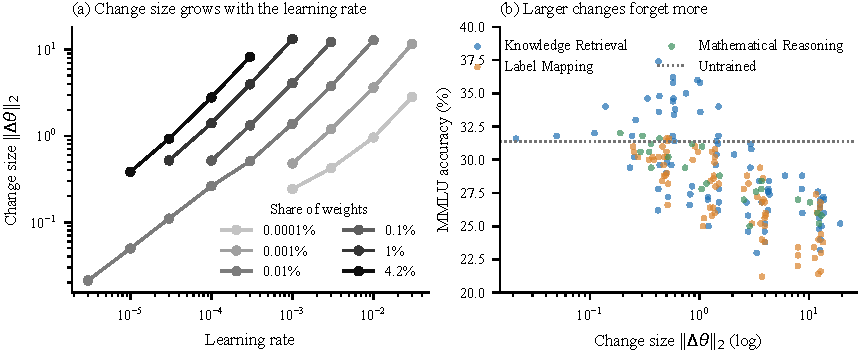
\includegraphics[width=\linewidth]{figures/f2_lr_change_forgetting.pdf}
  \caption{Learning rate, weight changes, and forgetting. Left: change size $\|\Delta\theta\|_2$ at each learning rate, grouped by the fraction of weights trained (log scales). Right: MMLU accuracy for each run, with the untrained model as a reference.}
  \label{fig:lr}
\end{figure}

\subsection{In-context performance is recovered with a tiny share of weights}

We found that updating a tiny percentage of weights during fine-tuning for CD can recover ICL performance across all three task-types. In both knowledge retrieval and label mapping, tuning 0.1\% of weights almost fully recovers ICL performance. In mathematical reasoning, updating 0.0001\% of weights, or 498 weights, already matches and slightly outperforms the teacher performance (Figure~\ref{fig:acc}).

\begin{figure}[t]
  \centering
  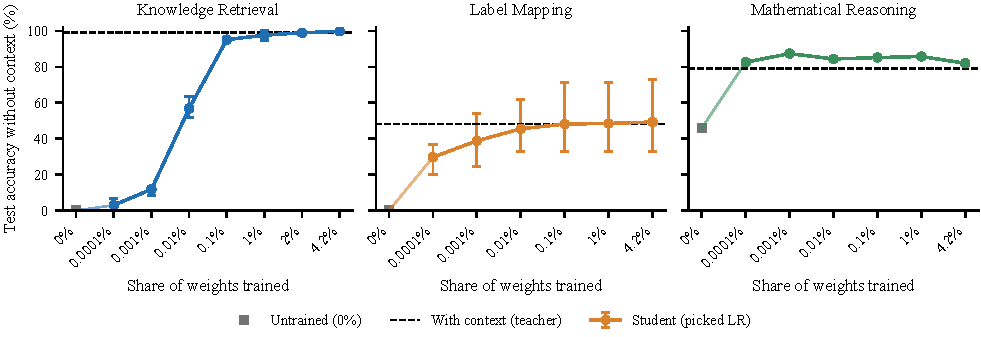
\includegraphics[width=\linewidth]{figures/f3_accuracy_by_share.pdf}
  \caption{Test accuracy after distillation. Learning rates are selected based on validation results. Points average three contexts; error bars show the range. Math uses one context. The horizontal axis lists the tested fractions of weights.}
  \label{fig:acc}
\end{figure}

\subsection{Forgetting stays small in MMLU and Mathematical Reasoning across Sparsity Levels}

We find that forgetfulness in MMLU stays close to the untrained model for Label Mapping and Mathematical Reasoning. However, Knowledge Retrieval experienced more forgetfulness with smaller shares of weights, but returns to the original performance for higher ones (Figure~\ref{fig:forget}). Mathematical Reasoning students drop $\sim$6-8 points at picked learning rates on MATH, but collapse at larger learning rates (Appendix~\ref{app:everylr}).

\begin{figure}[t]
  \centering
  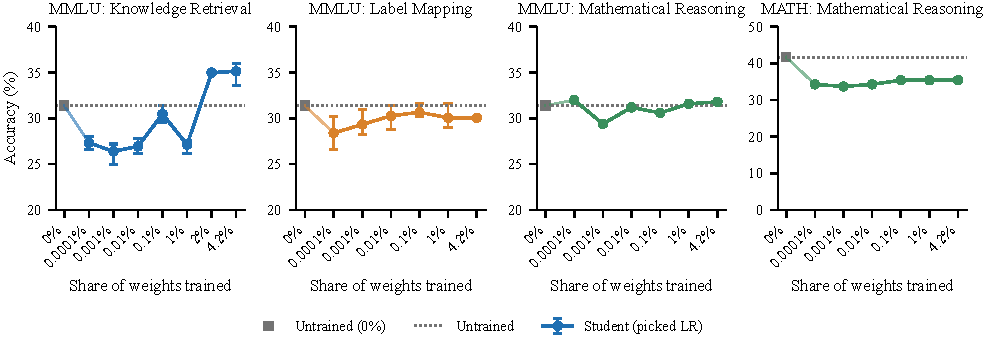
\includegraphics[width=\linewidth]{figures/f4_forgetting_by_share.pdf}
  \caption{Performance on MMLU and MATH after distillation, using learning rates chosen on validation data. Points are averaged over all  contexts; error bars show their range. Math uses one context. Dotted lines show performance before fine-tuning.}
  \label{fig:forget}
\end{figure}

\subsection{Savings in memory and inference compute}

Training memory at 4.2\% is about half that of full fine-tuning (6.2 vs 14.4 GB for Knowledge Retrieval, 8.8 vs 16.9 GB for Label Mapping). Full fine-tuning on Mathematical Reasoning ran out of memory on the 40 GB GPU even when restricted to the linear layers, while every share fit. Training time does not improve: every setting takes about one minute. At inference, students read 14× fewer input tokens per query for Knowledge Retrieval and Mathematical Reasoning, and 25× fewer for Label Mapping.

%\todo{At inference the student reads 14--25$\times$ fewer input tokens per query; training memory is
%about half of full fine-tuning; training time pending a controlled benchmark; full fine-tuning on Mathematical Reasoning ran out of memory on the 40 GB GPU. Memory and time barely change with the share.}
\begin{figure}[t]
  \centering
  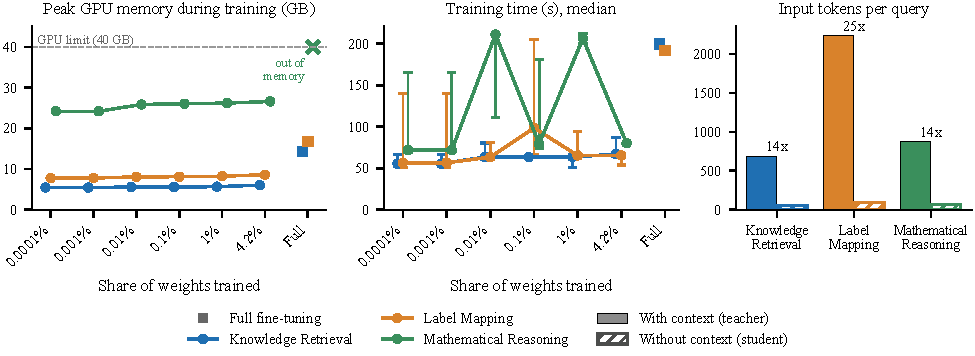
\includegraphics[width=\linewidth]{figures/f5_efficiency.pdf}
  \caption{Cost of training and inference. Left: peak training memory (dashed: 40 GB GPU limit; crosses: out of memory). Middle: training time, mean of 3 repeats on one A100 (bars: fastest and slowest repeat). Squares and triangles: full fine-tuning of all weights and of the linear layers only. Right: input tokens per query with the context (teacher) and without it (student).}
  \label{fig:cost}
\end{figure}
\begin{table}[t]
  \centering\small
  \begin{tabular}{llrrr}
\toprule
Task & Method & Trained (M) & Memory (GB) & Time (s) \\
\midrule
Knowledge Retrieval & Weights, 4.2\% & 20.7 & 6.2 & 61 \\
Knowledge Retrieval & Full, linear layers & 497.6 & 11.3 & 56 \\
Knowledge Retrieval & Full, all weights & 752.4 & 14.4 & 61 \\
\midrule
Label Mapping & Weights, 4.2\% & 20.7 & 8.8 & 65 \\
Label Mapping & Full, linear layers & 497.6 & 13.8 & 59 \\
Label Mapping & Full, all weights & 752.4 & 16.9 & 65 \\
\midrule
Mathematical Reasoning & Weights, 4.2\% & 20.7 & 26.6 & 77 \\
Mathematical Reasoning & Full, linear layers & 497.6 & \multicolumn{2}{c}{out of memory (40 GB)} \\
Mathematical Reasoning & Full, all weights & 752.4 & \multicolumn{2}{c}{out of memory (40 GB)} \\
\bottomrule
\end{tabular}

  \caption{Training memory and time at the 4.2\% budget and for full fine-tuning (mean of 3 repeats).}
  \label{tab:cost}
\end{table}

\subsection{Structured fine-tuning: weights, rows and blocks}

We find that at 4.2\%, updating individual weights and rows perform similarly across task-types, with blocks needing larger learning rates to learn Knowledge Retrieval and Label mapping. Blocks also forget significantly more in MMLU, with a score roughly equal to chance with the knowledge retrieval and Label Mapping students.

\begin{figure}[ht]
  \centering
  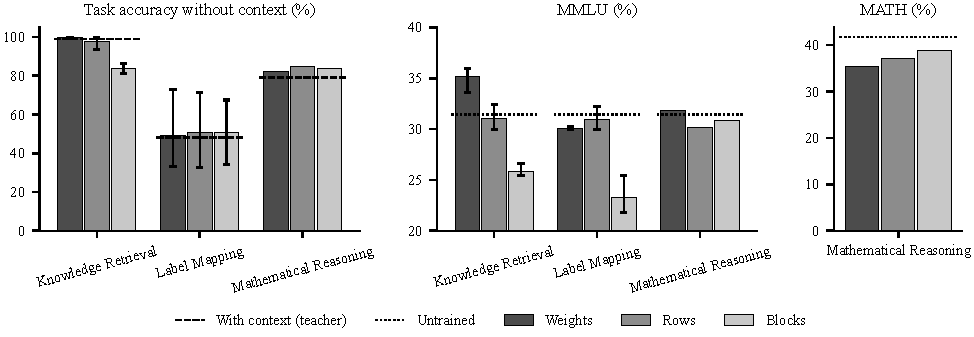
\includegraphics[width=\linewidth]{figures/f6_granularity.pdf}
  \caption{Updating individual weights, rows, or blocks at the same 4.2\% budget. Learning rates are tuned separately for weights, rows, and blocks. Bars illustrate the average over all contexts; error bars show their range. Math uses one context.}
  \label{fig:gran}
\end{figure}

\subsection{Top-gradient versus random selection}
\inprogress\ Same shares and learning-rate grid with a random mask.

% =====================================================================================================
\section{Discussion and limitations}
\label{sec:discussion}
Our results suggest that context distillation can recover much of the teacher's performance by updating a small fraction of weights. However, updating fewer weights does not prevent forgetting by itself. The learning rate is also important, and the fraction of weights needed also varies across the tasks we study.

These findings are limited to one 0.8B model and one random seed per setting. Our experiments for Mathematical Reasoning use only one context, teaching the digit-sum method for remainders modulo 9, so its results do not establish that other reasoning skills are equally easy to distill. Our forgetting measures also cover only a small part of the model's abilities. In particular, the untrained model scores about six percentage points above chance on MMLU with option-text scoring, leaving little room to measure further degradation. Staying close to this baseline does not establish that the model's broader abilities are preserved.

The comparisons also have practical limits. We search different learning-rate ranges at different parameter shares, so the results reflect both the number of weights updated and the rates we tried. They do not establish the best performance achievable at each share. The comparison with random weight selection is also still in progress, so we cannot yet determine how much of the benefit comes from selecting weights by gradient magnitude.

\section{Conclusion}
\label{sec:conclusion}
%\todo{Two or three sentences.}

Our experiments show that context distillation can recover much of the teacher’s performance while updating only a small fraction of the model’s weights. We also observe that learning rate strongly affects forgetting, so reducing the number of updated weights alone is not enough to preserve prior abilities. These results support selective fine-tuning as a practical approach to context distillation.

% =====================================================================================================
\small
\bibliographystyle{abbrvnat}
\bibliography{refs}

% =====================================================================================================
\clearpage
\appendix
\normalsize

\section{Task examples}
\label{app:tasks}
Table~\ref{tab:examples} shows an excerpt of one context per task and a test query. The teacher
sees the full context before the query, but the student sees only the query.
\begin{table}[h]
  \centering\small
  \begin{tabular}{p{2.2cm}p{5.6cm}p{3.6cm}l}
    \toprule
    Task & Context (excerpt) & Test query & Answer \\
    \midrule
    Knowledge Retrieval &
    \emph{Tenlun Triostlun was born in 1920 in the town of Trizarstead. Tenlun Triostlun works as a shipwright.} \dots &
    \emph{Where does Tenlun Triostlun come from originally?} & Trizarstead \\
    \addlinespace
    Label Mapping &
    \emph{Input: Insurance Probe Hits Home in DC Region \dots\ Label: cloud} \dots\ (World $\to$ river, Sports $\to$ stone, Business $\to$ cloud, Sci/Tech $\to$ lamp) &
    \emph{Input: Britain condemns bomb attack in Kathmandu \dots\ Label:} & river \\
    \addlinespace
    Mathematical Reasoning &
    \emph{What is the remainder when 487575745 is divided by 9? A number has the same remainder mod 9 as the
    sum of its digits. Digit sum: 4+8+\dots+5 = 52. 52 = 9 $\times$ 5 + 7. Answer: 7} \dots &
    \emph{What is the remainder when 531164237 is divided by 9?} & 5 \\
    \bottomrule
  \end{tabular}
  \caption{One context excerpt and test query per task.}
  \label{tab:examples}
\end{table}

\section{Every learning rate, per context}
\label{app:everylr}
\begin{figure}[h]
  \centering
  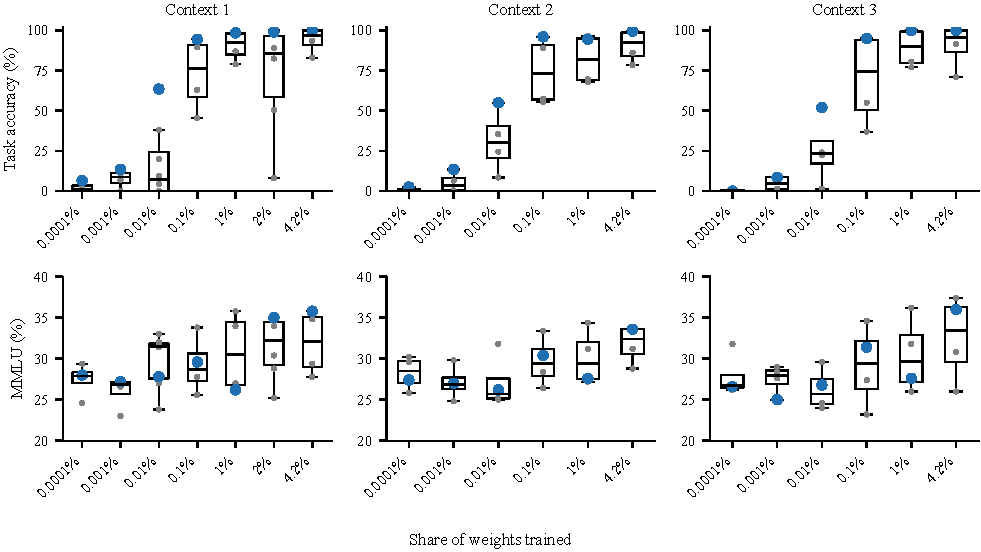
\includegraphics[width=\linewidth]{figures/f7_every_lr_knowledge.pdf}
  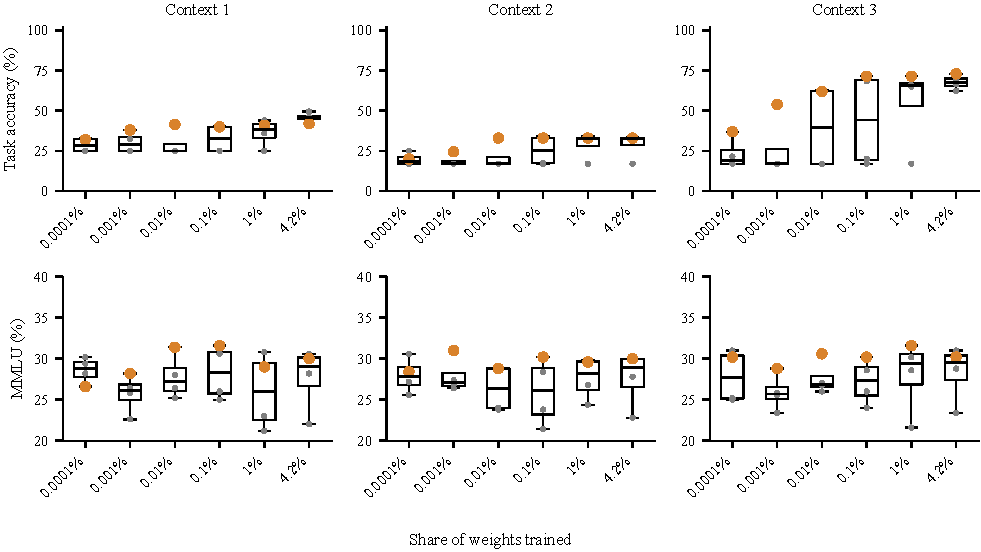
\includegraphics[width=\linewidth]{figures/f7_every_lr_arbitrary.pdf}
  \caption{Sensitivity to learning rate for each context and fraction of weights trained. Gray dots show individual runs; colored dots mark the chosen learning rate. Boxes show the median and middle 50\%; whiskers use the 1.5-IQR rule.}
  \label{fig:box}
\end{figure}
\begin{figure}[h]
  \centering
  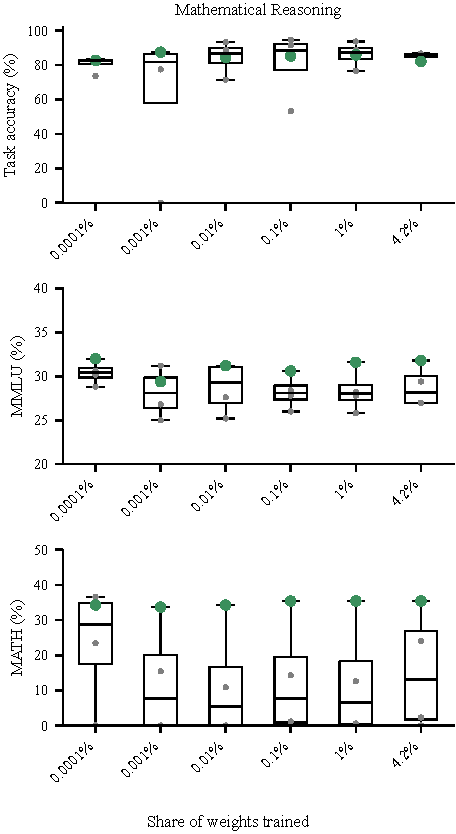
\includegraphics[width=0.5\linewidth]{figures/f7_every_lr_math.pdf}
  \caption{Learning-rate sensitivity for Mathematical Reasoning, measured by task accuracy, MMLU, and MATH. Plot conventions follow Figure~\ref{fig:box}.}
\end{figure}
\begin{table}[h]
  \centering\small
  \begin{tabular}{llrlrrr}
\toprule
Task & Share & Weights & LR & Accuracy & Recovery & MMLU \\
\midrule
Knowledge Retrieval & 0.0001\% & 498 & 1e-2 & 3.0\% & 3\% & 27.3\% \\
Knowledge Retrieval & 0.001\% & 4,976 & 3e-3 & 11.8\% & 12\% & 26.4\% \\
Knowledge Retrieval & 0.01\% & 49,761 & 1e-3 & 56.8\% & 57\% & 26.9\% \\
Knowledge Retrieval & 0.1\% & 497,615 & 3e-4 & 95.2\% & 96\% & 30.5\% \\
Knowledge Retrieval & 1\% & 4,976,148 & 3e-4 & 97.7\% & 99\% & 27.1\% \\
Knowledge Retrieval & 2\% & 9,952,297 & 3e-5 & 99.0\% & 99\% & 35.0\% \\
Knowledge Retrieval & 4.2\% & 20,733,952 & 3e-5 & 99.8\% & 101\% & 35.1\% \\
\midrule
Label Mapping & 0.0001\% & 498 & 3e-3 & 29.7\% & 31\% & 28.4\% \\
Label Mapping & 0.001\% & 4,976 & 1e-3 & 38.8\% & 60\% & 29.3\% \\
Label Mapping & 0.01\% & 49,761 & 3e-4 & 45.5\% & 87\% & 30.3\% \\
Label Mapping & 0.1\% & 497,615 & 1e-4 & 48.2\% & 93\% & 30.7\% \\
Label Mapping & 1\% & 4,976,148 & 3e-5 & 48.5\% & 94\% & 30.1\% \\
Label Mapping & 4.2\% & 20,733,952 & 1e-5 & 49.3\% & 97\% & 30.1\% \\
\midrule
Mathematical Reasoning & 0.0001\% & 498 & 1e-3 & 82.6\% & 110\% & 32.0\% \\
Mathematical Reasoning & 0.001\% & 4,976 & 1e-3 & 87.4\% & 125\% & 29.4\% \\
Mathematical Reasoning & 0.01\% & 49,761 & 3e-4 & 84.4\% & 116\% & 31.2\% \\
Mathematical Reasoning & 0.1\% & 497,615 & 1e-4 & 85.2\% & 118\% & 30.6\% \\
Mathematical Reasoning & 1\% & 4,976,148 & 3e-5 & 85.8\% & 120\% & 31.6\% \\
Mathematical Reasoning & 4.2\% & 20,733,952 & 1e-5 & 82.0\% & 108\% & 31.8\% \\
\bottomrule
\end{tabular}

  \caption{Test results at the learning rate chosen for each task and fraction of weights. Scores are averaged across contexts; recovery is defined in Eq.~\ref{eq:recovery}.}
\end{table}

\section{Training curves}
\label{app:curves}
\begin{figure}[h]
  \centering
  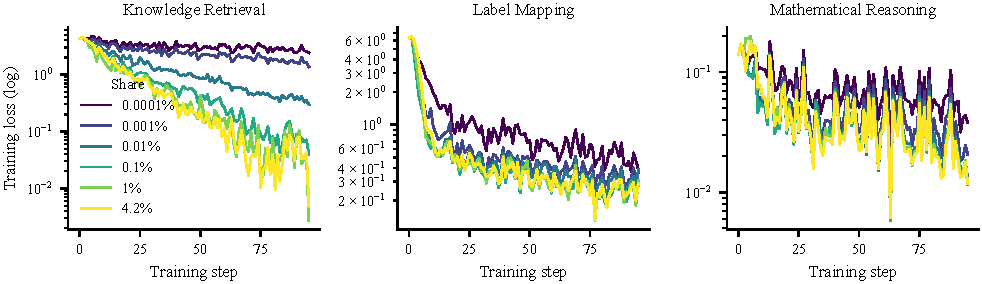
\includegraphics[width=\linewidth]{figures/f8_training_loss.pdf}
  \caption{Training loss for each fraction of weights, using learning rates chosen on validation data. Curves average contexts; math uses one context. Loss is shown on a log scale.}
\end{figure}

\section{Why MMLU is scored by option text}
\label{app:mmlu}
We first scored MMLU by the probability of the answer letter (A--D). Some Label Mapping students then
scored far below chance because they had learned to begin every answer with a label word, so the letter
probability carried almost no mass (e.g.\ the top first token was ``orange'' 99.8\% of the time). This is
a change in answer format and not lost knowledge. Scored by option text (Eq.~\ref{eq:mmlu}), the same
student reached 30.8\% versus 31.4\% for the untrained model. We therefore score all models by option text.

\section{Learning-rate grids and pilot}
\label{app:hparams}
A pilot on one context per task, at shares of 0.01\% and 2\% with six learning rates (3e-6 to 1e-3), showed that smaller shares need larger learning rates (best at $\geq$1e-3 for 0.01\% and about 1e-4 for 2\% on Knowledge Retrieval). We therefore gave each share its own grid of four rates in steps of 3$\times$, shifted up as the share shrinks (Table~\ref{tab:hparams}). For Label Mapping and Mathematical Reasoning the picked rate is often the lowest of its grid, so a smaller rate might forget even less; we plan to list this as a limitation.

\section{Compute}
All runs used one A100-40GB GPU each. We trained 240 models: 178 for the share sweep, 56 with rows or
blocks, and 6 with full fine-tuning (full fine-tuning on Mathematical Reasoning did not fit in memory).
A training run takes about one minute on average.

\section{Github Repository}

Our Github Repository containing the code can be found here. The results for the tables in this paper can be found in the paper-and-results branch: 

https://github.com/Nazarshia2889/Selective-Fine-Tuning-for-Context-Distillation

\end{document}
